This section describes how an application, the SYCL runtime library, and the GPU software driver work together to offload a kernel on GPU hardware. The diagram in Figure 15-14 shows a typical software stack with these layers of abstraction. In many cases, the existence of these layers is transparent to an application, but it is important to understand and account for them when debugging or profiling our application.\par

\hspace*{\fill} \par %插入空行
Figure 15-14. Offloading parallel kernels to GPUs (simplified)
\begin{center}
	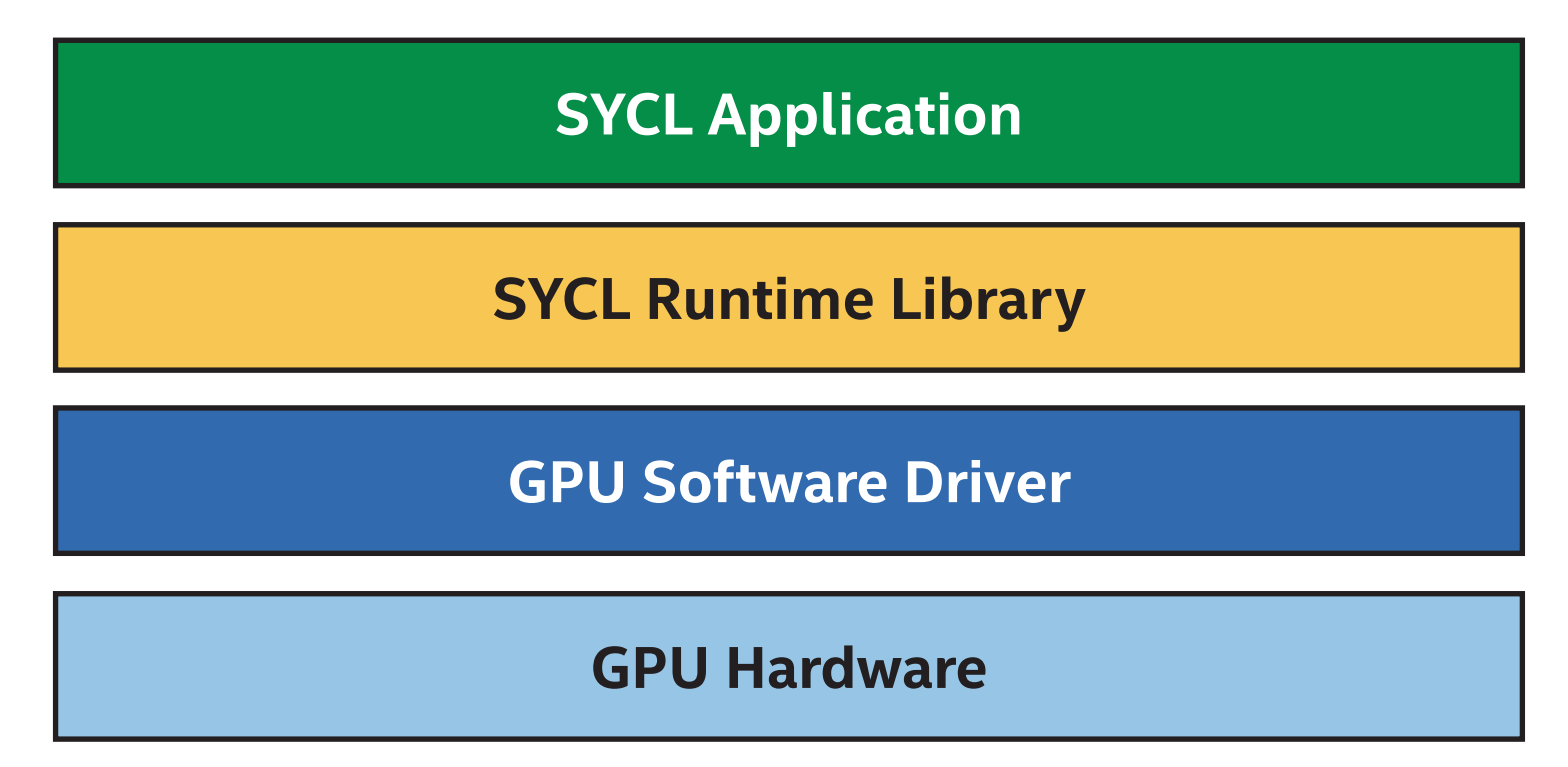
\includegraphics[width=1.0\textwidth]{content/chapter-15/images/10}
\end{center}

\hspace*{\fill} \par %插入空行
\textbf{SYCL Runtime Library}

The SYCL runtime library is the primary software library that SYCL applications interface with. The runtime library is responsible for implementing classes such as queues, buffers, and accessors and the member functions of these classes. Parts of the runtime library may be in header files and hence directly compiled into the application executable. Other parts of the runtime library are implemented as library functions, which are linked with the application executable as part of the application build process. The runtime library is usually not device-specific, and the same runtime library may orchestrate offload to CPUs, GPUs, FPGAs, or other devices.\par

\hspace*{\fill} \par %插入空行
\textbf{GPU Software Drivers}

Although it is theoretically possible that a SYCL runtime library could offload directly to a GPU, in practice, most SYCL runtime libraries interface with a GPU software driver to submit work to a GPU.\par

A GPU software driver is typically an implementation of an API, such as OpenCL, Level Zero, or CUDA. Most of a GPU software driver is implemented in a user-mode driver library that the SYCL runtime calls into, and the user-mode driver may call into the operating system or a kernel-mode driver to perform system-level tasks such as allocating memory or submitting work to the device. The user-mode driver may also invoke other user-mode libraries; for example, the GPU driver may invoke a GPU compiler to just-in-time compile a kernel from an intermediate representation to GPU ISA (Instruction Set Architecture). These software modules and the interactions between them are shown in Figure 15-15.\par

\hspace*{\fill} \par %插入空行
Figure 15-15. Typical GPU software driver modules
\begin{center}
	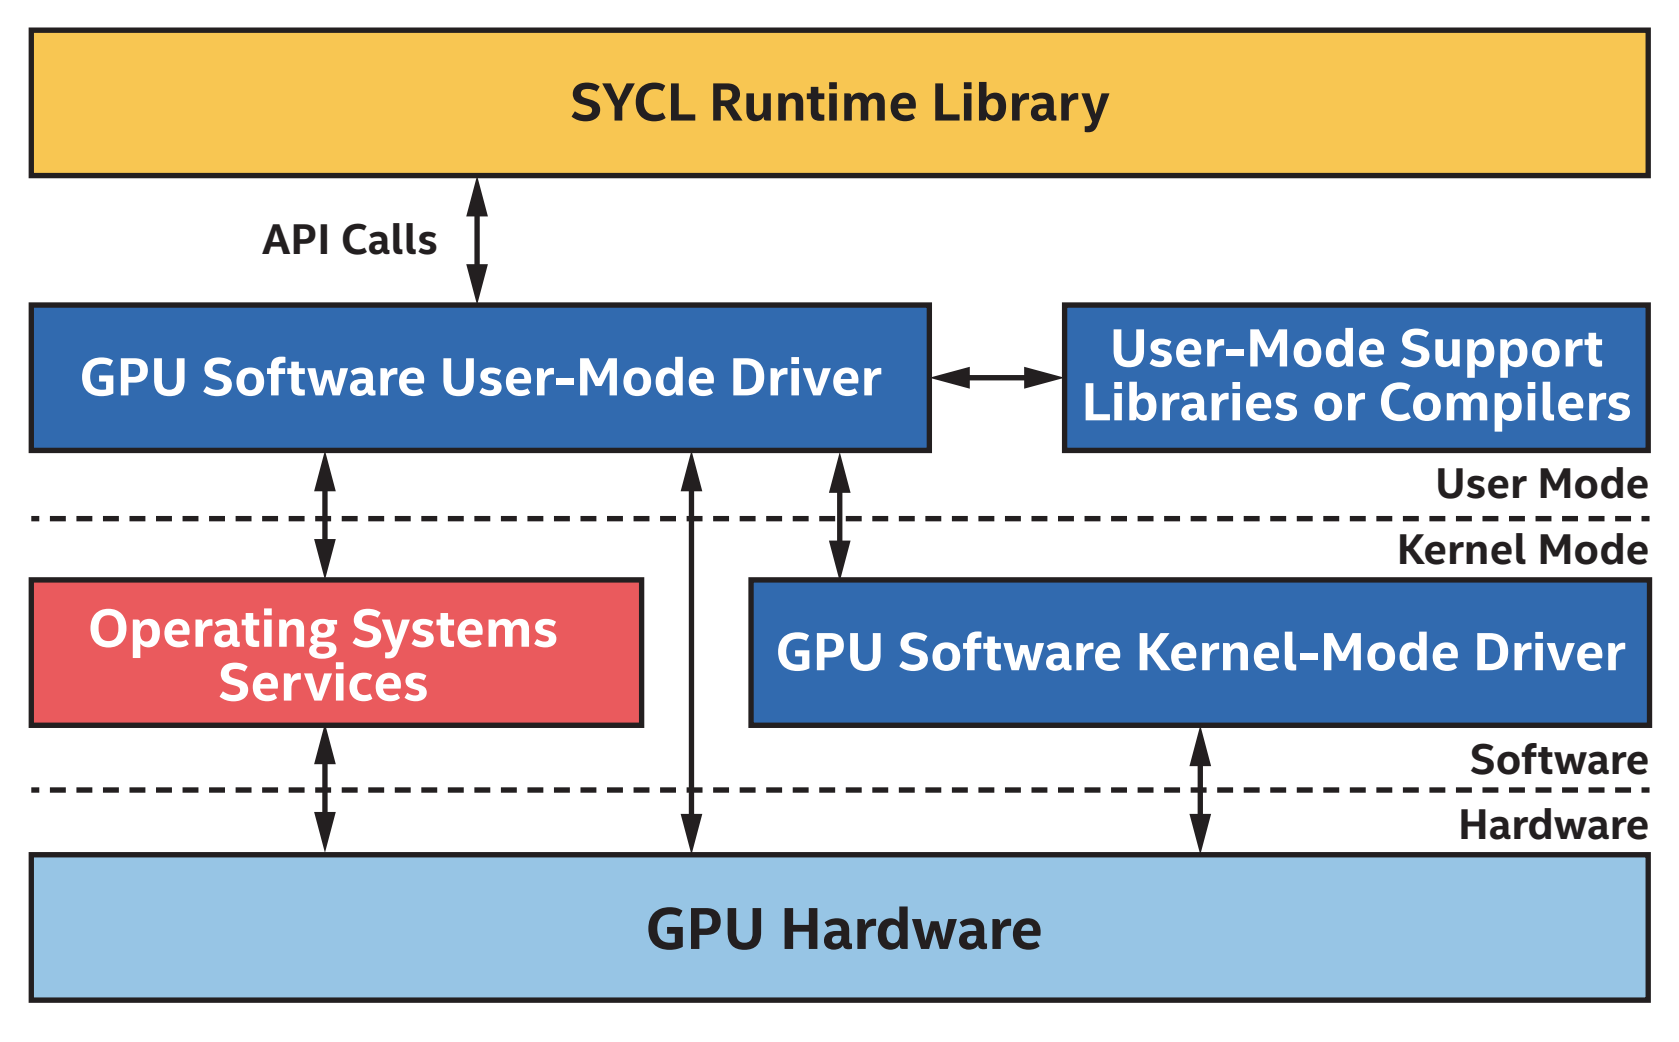
\includegraphics[width=1.0\textwidth]{content/chapter-15/images/11}
\end{center}

\hspace*{\fill} \par %插入空行
\textbf{GPU Hardware}

When the runtime library or the GPU software user-mode driver is explicitly requested to submit work or when the GPU software heuristically determines that work should begin, it will typically call through the operating system or a kernel-mode driver to start executing work on the GPU. In some cases, the GPU software user-mode driver may submit work directly to the GPU, but this is less common and may not be supported by all devices or operating systems.\par

When the results of work executed on a GPU are consumed by the host processor or another accelerator, the GPU must issue a signal to indicate that work is complete. The steps involved in work completion are very similar to the steps for work submission, executed in reverse: the GPU may signal the operating system or kernel-mode driver that it has finished execution, then the user-mode driver will be informed, and finally the runtime library will observe that work has completed via GPU software API calls.\par

Each of these steps introduces latency, and in many cases, the runtime library and the GPU software are making a tradeoff between lower latency and higher throughput. For example, submitting work to the GPU more frequently may reduce latency, but submitting frequently may also reduce throughput due to per-submission overheads. Collecting large batches of work increases latency but amortizes submission overheads over more work and introduces more opportunities for parallel execution. The runtime and drivers are tuned to make the right tradeoff and usually do a good job, but if we suspect that driver heuristics are submitting work inefficiently, we should consult documentation to see if there are ways to override the default driver behavior using API-specific or even implementation-specific mechanisms.\par

\hspace*{\fill} \par %插入空行
\textbf{Beware the Cost of Offloading!}

Although SYCL implementations and GPU vendors are continually innovating and optimizing to reduce the cost of offloading work to a GPU, there will always be overhead involved both when starting work on a GPU and observing results on the host or another device. When choosing where to execute an algorithm, consider both the benefit of executing an algorithm on a device and the cost of moving the algorithm and any data that it requires to the device. In some cases, it may be most efficient to perform a parallel operation using the host processor—or to execute a serial part of an algorithm inefficiently on the GPU—to avoid the overhead of moving an algorithm from one processor to another.\par

\begin{tcolorbox}[colback=red!5!white,colframe=red!75!black]
Consider the performance of our algorithm as a whole—it may be most efficient to execute part of an algorithm inefficiently on one device than to transfer execution to another device!
\end{tcolorbox}

\hspace*{\fill} \par %插入空行
\textbf{Transfers to and from Device Memory}

On GPUs with dedicated memory, be especially aware of transfer costs between dedicated GPU memory and memory on the host or another device. Figure 15-16 shows typical memory bandwidth differences between different memory types in a system.\par

\hspace*{\fill} \par %插入空行
Figure 15-16. Typical differences between device memory, remote memory, and host memory
\begin{center}
	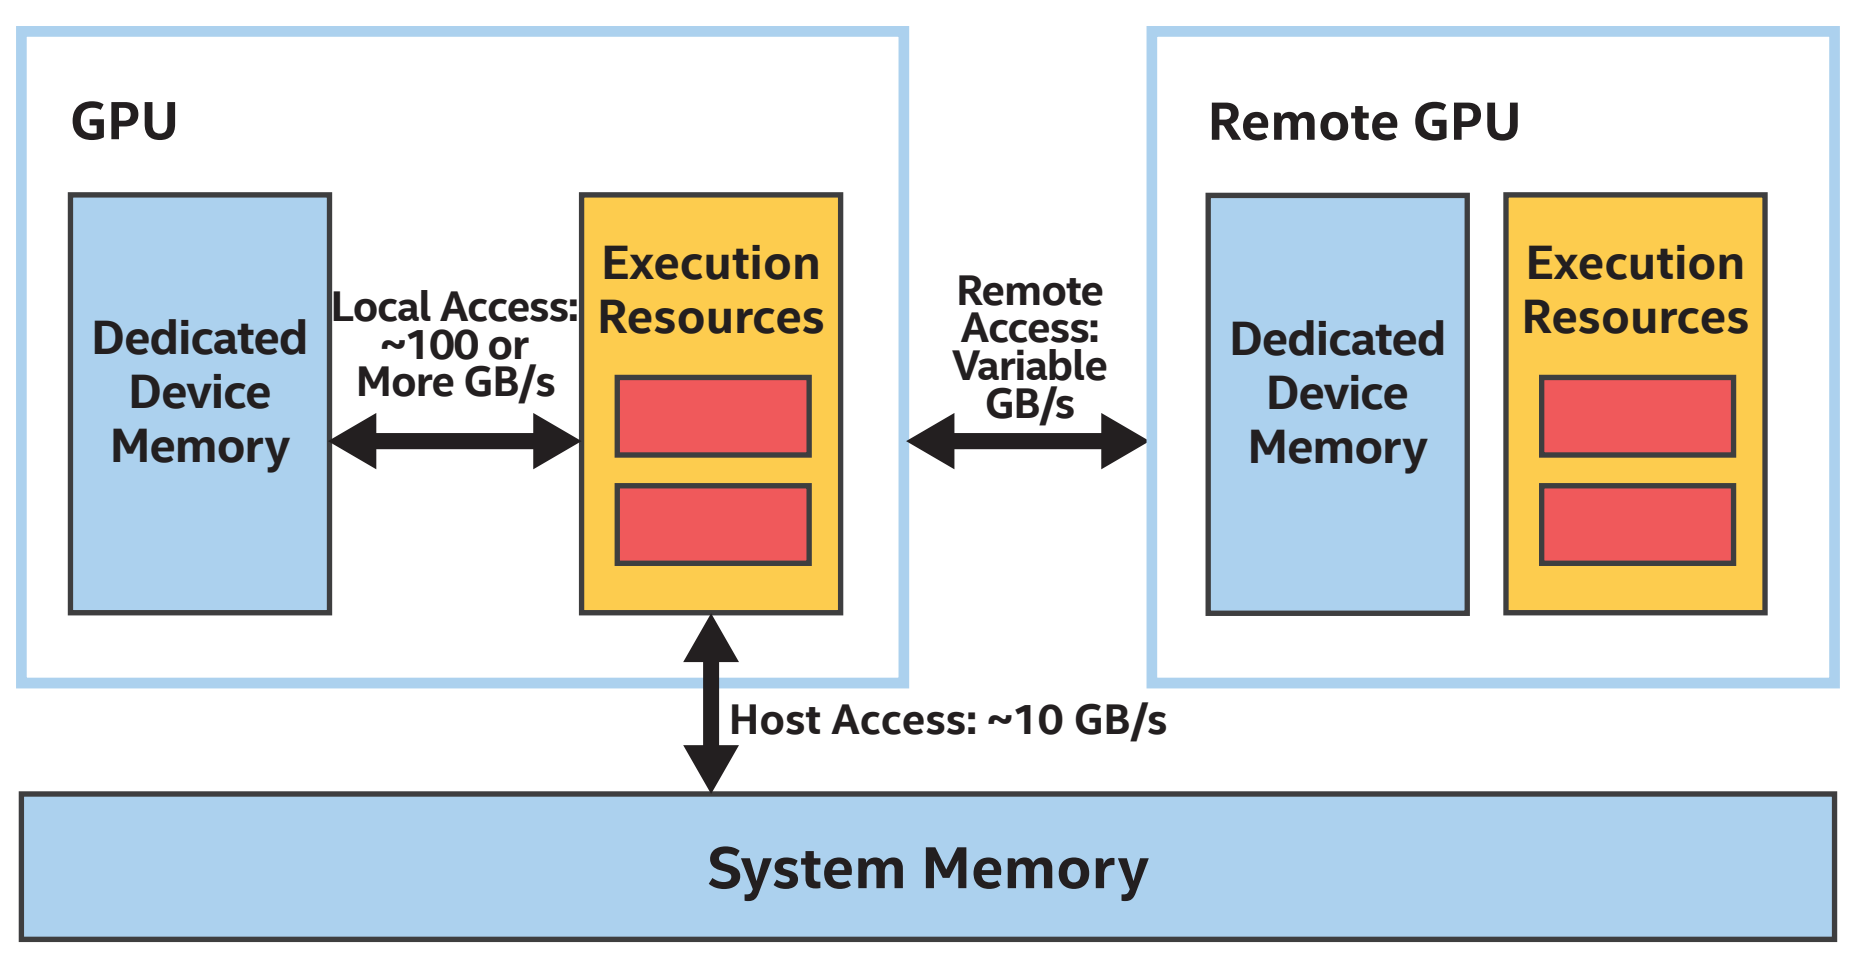
\includegraphics[width=1.0\textwidth]{content/chapter-15/images/12}
\end{center}

Recall from Chapter 3 that GPUs prefer to operate on dedicated device memory, which can be faster by an order of magnitude or more, instead of operating on host memory or another device’s memory. Even though accesses to dedicated device memory are significantly faster than accesses to remote memory or system memory, if the data is not already in dedicated device memory then it must be copied or migrated.\par

So long as the data will be accessed frequently, moving it into dedicated device memory is beneficial, especially if the transfer can be performed asynchronously while the GPU execution resources are busy processing another task. When the data is accessed infrequently or unpredictably though, it may preferable to save transfer costs and operate on the data remotely or in system memory, even if per-access costs are higher. Chapter 6 describes ways to control where memory is allocated and different techniques to copy and prefetch data into dedicated device memory. These techniques are important when optimizing program execution for GPUs.\par








